\documentclass{../khlslides}


\title[Functies]{Functies}
\author{Fr\'ed\'eric Vogels}


\pgfkeys{/tikz/flowchart/node/.style={rectangle,fill=blue,opacity=0.5,text opacity=1,drop shadow,inner sep=2mm}}
\pgfkeys{/tikz/flowchart/arrow/.style={-latex,flowchart/arrowline}}
\pgfkeys{/tikz/flowchart/arrowline/.style={thick}}


\newcommand{\lcurly}{{\tt{\char '173}}}
\newcommand{\link}[2]{\href{#1}{\beamergotobutton{#2}}}
\newcommand{\PLACEHOLDER}[1]{\ensuremath{\langle}\textrm{\textit{#1}\ensuremath{\rangle}}}


\pgfkeys{
  /wof/sequence point/.cd,
  placement/.initial=above,
  rotation/.initial=0,
  /wof/sequence link/.cd,
  label/.initial={},
  /wof/round/.cd,
  name prefix/.initial=,
  /tikz/.cd,
  sequence point/.style={blue!50,thick,fill=white},
  sequence point label/.style={font=\tiny,black},
  sequence link/.style={blue!50,thick},
  active/.style={fill=red,thick,red}
}
\newcommand<>{\seqpoint}[3][]{
  \only#4{{
  \pgfkeys{/wof/sequence point/.cd,#1}
  \pgfkeys{/wof/sequence point/placement/.get=\placement}
  \pgfkeys{/wof/sequence point/rotation/.get=\rotation}
  \draw[sequence point] (#2) circle (.05)
                        node[sequence point label,\placement,rotate=\rotation] {#3};
}}}
\newcommand<>{\seqlink}[3][]{\only#4{{
  \pgfkeys{/wof/sequence link/.cd,#1}
  \pgfkeys{/wof/sequence link/label/.get=\seqlinklabel}
  \draw[sequence link] (#2) -- (#3) node[midway,sloped,yshift=1mm,font=\tiny,black] {\seqlinklabel};
}}}


\begin{document}

\begin{frame}
  \titlepage
\end{frame}

\begin{frame}
  \frametitle{Rad van Fortuin}

  \begin{center}
    \begin{tikzpicture}
      \path[use as bounding box] (0,-2) rectangle (8,4);

      \coordinate (init) at (0,0);
      \coordinate (turn wheel) at ($ (init) + (1,2) $);
      \coordinate (bankruptcy lose money) at ($ (turn wheel) + (1,1.5) $);
      \coordinate (bankruptcy next player) at ($ (bankruptcy lose money) + (2,0) $);
      \coordinate (pass) at ($ (turn wheel) + (3,0.5) $);
      \coordinate (joker) at ($ (turn wheel) + (3,-0.5) $);
      \coordinate (consonant) at ($ (turn wheel) + (1,-2) $);
      \coordinate (show consonant) at ($ (consonant) + (1,0) $);
      \coordinate (gain) at ($ (show consonant) + (1,0.5) $);
      \coordinate (no consonants) at ($ (show consonant) + (1,-0.5) $);
      \coordinate (end consonants) at ($ (show consonant) + (2,0) $);
      \coordinate (vowel) at ($ (init) + (1,-2) $);
      \coordinate (buy vowel) at ($ (vowel) + (1.5,0) $);
      \coordinate (show vowels) at ($ (buy vowel) + (1.5,0) $);
      \coordinate (no vowels) at ($ (show vowels) + (1,.5) $);
      \coordinate (end vowels) at ($ (show vowels) + (2,0) $);
      \coordinate (exit) at ($ (init) + (8,0) $);

      \seqlink[label=rad]{init}{turn wheel}
      \seqlink[label=bankroet]{turn wheel}{bankruptcy lose money}
      \seqlink{bankruptcy lose money}{bankruptcy next player}
      \seqlink[label=verlies beurt]{turn wheel}{pass}
      \seqlink[label=joker]{turn wheel}{joker}
      \seqlink[label=else]{turn wheel}{consonant}
      \seqlink{consonant}{show consonant}
      \seqlink[label=0]{show consonant}{no consonants}
      \seqlink[label=1+]{show consonant}{gain}
      \seqlink{gain}{end consonants}
      \seqlink{no consonants}{end consonants}
      \seqlink{end consonants}{exit}
      \seqlink{joker}{exit}
      \seqlink{pass}{exit}
      \seqlink{bankruptcy next player}{exit}
      \seqlink[label=klinker]{init}{vowel}
      \seqlink{vowel}{buy vowel}
      \seqlink{buy vowel}{show vowels}
      \seqlink[label=0]{show vowels}{no vowels}
      \seqlink{no vowels}{end vowels}
      \seqlink[label=1+]{show vowels}{end vowels}
      \seqlink{end vowels}{exit}

      \draw[sequence link,-latex] (exit) -- +(0,-3) node[midway,sloped,black,yshift=1mm,font=\tiny] {!spel gedaan} -| ($ (init) + (0,-.2) $);
      \draw[sequence link,-latex] (exit) -- +(2,0) node[midway,sloped,black,yshift=1mm,font=\tiny] {spel gedaan};

      \seqpoint[placement=above left]{init}{rad/klinker}
      \seqpoint[placement=left]{turn wheel}{draai rad}
      \seqpoint{bankruptcy lose money}{score = 0}
      \seqpoint<1-2>{bankruptcy next player}{huidigeSpeler++}
      \seqpoint<3->[rotation=-12]{bankruptcy next player}{huidigeSpeler = (huidigeSpeler + 1) \% aantalSpelers}
      \seqpoint<1-2>{pass}{huidigeSpeler++}
      \seqpoint<3->[rotation=5]{pass}{huidigeSpeler = (huidigeSpeler + 1) \% aantalSpelers}
      \seqpoint{joker}{jokers++}
      \seqpoint[placement=below]{consonant}{gok medeklinker}
      \seqpoint{show consonant}{toon}
      \seqpoint{gain}{score += bedrag * k}
      \seqpoint<1-2>[placement=below]{no consonants}{huidigeSpeler++}
      \seqpoint<3->[placement=below]{no consonants}{huidigeSpeler = (huidigeSpeler + 1) \% aantalSpelers}
      \seqpoint{end consonants}{}
      \seqpoint[placement=below]{vowel}{gok klinker}
      \seqpoint[placement=below]{buy vowel}{score -= 50}
      \seqpoint[placement=below]{show vowels}{toon}
      \seqpoint<1-2>{no vowels}{huidigeSpeler++}
      \seqpoint<3->{no vowels}{huidigeSpeler = (huidigeSpeler + 1) \% aantalSpelers}
      \seqpoint{end vowels}{}
      \seqpoint{exit}{}


      \only<2>{
        \node[/khl/note,anchor=south west] (note next player correction) at ($ (bankruptcy next player) + (-5,.5) $) {\parbox{11cm}{\raggedright Moet eigenlijk \\ {\tt huidigeSpeler = (huidigeSpeler + 1) \% aantalSpelers} \\ zijn}};
        \draw[/khl/note arrow] (note next player correction) to[bend left=30] (bankruptcy next player);
        \draw[/khl/note arrow] (note next player correction) to[bend left=30] (pass);
        \draw[/khl/note arrow] (note next player correction) to[bend left=30] (no consonants);
        \draw[/khl/note arrow] (note next player correction) to[bend left=30] (no vowels);
      }

      \only<4-9>{
        \node[/khl/note,anchor=south] (note consonants) at ($ (consonant) + (0,.5) $) {\parbox{5cm}{\raggedright Checken dat het wel een medeklinker is, zoniet beurtverlies}};
        \draw[/khl/note arrow] (note consonants) to[bend left=30] (consonant);
      }

      \only<5-9>{
        \node[/khl/note,anchor=south] (note vowels) at ($ (vowel) + (0,.5) $) {\parbox{5cm}{\raggedright Checken dat het wel een klinker is, zoniet beurtverlies}};
        \draw[/khl/note arrow] (note vowels) to[bend left=30] (vowel);
      }

      \only<6-9>{
        \node[/khl/note,anchor=north] (note vowels sufficient money) at ($ (vowel) + (2,-.5) $) {\parbox{8cm}{\raggedright Checken dat speler genoeg geld heeft, zoniet verliesbeurt}};
        \draw[/khl/note arrow] (note vowels sufficient money.north) to[bend right=30] (vowel);
      }

      \only<7-9>{
        \node[/khl/note,anchor=south] (note time) at ($ (vowel) + (5,1.5) $) {\parbox{3cm}{\raggedright Moet ook nog binnen de tijd}};
        \draw[/khl/note arrow] (note time.west) to[bend left=30] (consonant);
        \draw[/khl/note arrow] (note time) to[bend left=30] (vowel);
      }

      \only<8-9>{
        \node[/khl/note,anchor=south] (note joker usage) at ($ (exit) + (0,0.5) $) {\parbox{3cm}{\raggedright Mogelijkheid om joker te gebruiken}};
        \draw[/khl/note arrow] (note joker usage) to[bend left=30] (exit);
      }

      \only<9>{
        \node[/khl/note] at (4,4) {\Huge Kortom: het wordt chaotisch};
      }
    \end{tikzpicture}
  \end{center}
\end{frame}

\begin{frame}
  \frametitle{Rad van Fortuin}

  \begin{center}
    \begin{tikzpicture}
      \path[use as bounding box] (0,-2) rectangle (8,4);

      \coordinate (init) at (0,0);
      \coordinate (turn wheel) at ($ (init) + (1,2) $);
      \coordinate (bankruptcy lose money) at ($ (turn wheel) + (1,1.5) $);
      \coordinate (bankruptcy next player) at ($ (bankruptcy lose money) + (2,0) $);
      \coordinate (bankruptcy call) at ($ (bankruptcy lose money) + (2,0) $);
      \coordinate (pass) at ($ (turn wheel) + (3,0.5) $);
      \coordinate (joker) at ($ (turn wheel) + (3,-0.5) $);
      \coordinate (consonant) at ($ (turn wheel) + (1,-2) $);
      \coordinate (show consonant) at ($ (consonant) + (1,0) $);
      \coordinate (consonant call) at ($ (joker) + (0,-1.5) $);
      \coordinate (gain) at ($ (show consonant) + (1,0.5) $);
      \coordinate (no consonants) at ($ (show consonant) + (1,-0.5) $);
      \coordinate (end consonants) at ($ (show consonant) + (2,0) $);
      \coordinate (vowel) at ($ (init) + (1,-2) $);
      \coordinate (buy vowel) at ($ (vowel) + (1.5,0) $);
      \coordinate (show vowels) at ($ (buy vowel) + (1.5,0) $);
      \coordinate (no vowels) at ($ (show vowels) + (1,.5) $);
      \coordinate (end vowels) at ($ (show vowels) + (2,0) $);
      \coordinate (turn wheel function) at ($ (init) + (4,1) $);
      \coordinate (guess vowel function) at ($ (init) + (4,-1) $);
      \coordinate (play turn) at ($ (init) ! .5 ! (exit) $);
      \coordinate (play game) at (play turn);
      \coordinate (exit) at ($ (init) + (8,0) $);

      \seqlink<1-6>[label=rad]{init}{turn wheel}
      \seqlink<1-2>[label=bankroet]{turn wheel}{bankruptcy lose money}
      \seqlink<3-6>[label=bankroet]{turn wheel}{bankruptcy call}
      \seqlink<3-6>{bankruptcy call}{exit}
      \seqlink<1-2>{bankruptcy lose money}{bankruptcy next player}
      \seqlink<1-6>[label=verlies beurt]{turn wheel}{pass}
      \seqlink<1-6>[label=joker]{turn wheel}{joker}
      \seqlink<1-5>[label=else]{turn wheel}{consonant}
      \seqlink<1-5>{consonant}{show consonant}
      \seqlink<1-5>[label=0]{show consonant}{no consonants}
      \seqlink<1-5>[label=1+]{show consonant}{gain}
      \seqlink<1-5>{gain}{end consonants}
      \seqlink<1-5>{no consonants}{end consonants}
      \seqlink<1-5>{end consonants}{exit}
      \seqlink<6>[label=else]{turn wheel}{consonant call}
      \seqlink<6>{consonant call}{exit}
      \seqlink<7-8>[label=rad]{init}{turn wheel function}
      \seqlink<7-8>{turn wheel function}{exit}
      \seqlink<1-6>{joker}{exit}
      \seqlink<1-6>{pass}{exit}
      \seqlink<1-2>{bankruptcy next player}{exit}
      \seqlink<1-7>[label=klinker]{init}{vowel}
      \seqlink<1-7>{vowel}{buy vowel}
      \seqlink<1-7>{buy vowel}{show vowels}
      \seqlink<1-7>[label=0]{show vowels}{no vowels}
      \seqlink<1-7>{no vowels}{end vowels}
      \seqlink<1-7>[label=1+]{show vowels}{end vowels}
      \seqlink<1-7>{end vowels}{exit}
      \seqlink<8>[label=klinker]{init}{guess vowel function}
      \seqlink<8>{guess vowel function}{exit}
      \seqlink<9>{init}{play turn}
      \seqlink<9>{play turn}{exit}
      \seqlink<10>{init}{play game}
      \seqlink<10>{play game}{exit}

      \only<1-9>{
        \draw[sequence link,-latex] (exit) -- +(0,-3) node[midway,sloped,black,yshift=1mm,font=\tiny] {!spel gedaan} -| ($ (init) + (0,-.2) $);
        \draw[sequence link,-latex] (exit) -- +(2,0) node[midway,sloped,black,yshift=1mm,font=\tiny] {spel gedaan};
      }

      \seqpoint<1-8>[placement=above left]{init}{rad/klinker}
      \seqpoint<9>{init}{}
      \seqpoint<1-6>[placement=left]{turn wheel}{draai rad}
      \seqpoint<1-2>{bankruptcy lose money}{score = 0}
      \seqpoint<3-6>{bankruptcy call}{behandel bankroet}
      \seqpoint<1>[rotation=-12]{bankruptcy next player}{huidigeSpeler = (huidigeSpeler + 1) \% aantalSpelers}
      \seqpoint<2>{bankruptcy next player}{volgende speler}
      \seqpoint<1>[rotation=5]{pass}{huidigeSpeler = (huidigeSpeler + 1) \% aantalSpelers}
      \seqpoint<2-3>{pass}{volgende speler}
      \seqpoint<4-6>{pass}{behandel verliesbeurt}
      \seqpoint<1-4>{joker}{jokers++}
      \seqpoint<5-6>{joker}{behandel joker}
      \seqpoint<1-5>[placement=below]{consonant}{gok medeklinker}
      \seqpoint<1-5>{show consonant}{toon}
      \seqpoint<1-5>{gain}{score += bedrag * k}
      \seqpoint<1>[placement=below]{no consonants}{huidigeSpeler = (huidigeSpeler + 1) \% aantalSpelers}
      \seqpoint<2-5>[placement=below]{no consonants}{volgende speler}
      \seqpoint<1-5>{end consonants}{}
      \seqpoint<6>[placement=below]{consonant call}{behandel medeklinker}
      \seqpoint<7-8>{turn wheel function}{draai het rad}
      \seqpoint<1-7>[placement=below]{vowel}{gok klinker}
      \seqpoint<1-7>[placement=below]{buy vowel}{score -= 50}
      \seqpoint<1-7>[placement=below]{show vowels}{toon}
      \seqpoint<1>{no vowels}{huidigeSpeler = (huidigeSpeler + 1) \% aantalSpelers}
      \seqpoint<2-7>{no vowels}{volgende speler}
      \seqpoint<1-7>{end vowels}{}
      \seqpoint<8>{guess vowel function}{koop klinker}
      \seqpoint<9>{play turn}{speel beurt}
      \seqpoint<10>{play game}{speel spel}
      \seqpoint<1-9>{exit}{}

      \coordinate (next player init) at (6,4.5);
      \coordinate (next player inc) at ($ (next player init) + (1,0) $);
      \coordinate (next player exit) at ($ (next player inc) + (1,0) $);
      \seqlink<2>{next player init}{next player inc}
      \seqlink<2>{next player inc}{next player exit}
      \seqpoint<2>{next player inc}{huidigeSpeler = (huidigeSpeler + 1) \% aantalSpelers}
      \only<2>{
        \draw[black] ($ (next player init) + (-1.5,-.25) $) rectangle ($ (next player exit) + (1.5,.5) $);
        \node[anchor=north] at ($ (next player inc) + (0,-.25) $) {\tiny volgende speler};
      }

      \coordinate (bankrupt function init) at (6,4.5);
      \coordinate (bankrupt function reset score) at ($ (bankrupt function init) + (1,0) $);
      \coordinate (bankrupt function next player) at ($ (bankrupt function reset score) + (1,0) $);
      \coordinate (bankrupt function exit) at ($ (bankrupt function next player) + (1,0) $);
      \seqlink<3>{bankrupt function init}{bankrupt function reset score};
      \seqlink<3>{bankrupt function reset score}{bankrupt function next player};
      \seqlink<3>{bankrupt function next player}{bankrupt function exit};
      \seqpoint<3>{bankrupt function reset score}{score = 0};
      \seqpoint<3>[placement=below]{bankrupt function next player}{volgende speler};
      \only<3->{
        \draw[black] ($ (bankrupt function init) + (-.5,-.5) $) rectangle ($ (bankrupt function exit) + (.5,.5) $);
      }
      \only<4->{
        \node at ($ (bankrupt function init) ! .5 ! (bankrupt function exit) $) {\dots};
      }

      \only<3>{
        \node[anchor=north] at ($ (bankrupt function init) ! .5 ! (bankrupt function exit) + (0,-.5) $) {\tiny behandel bankroet};
      }
      \only<4>{
        \node[anchor=north] at ($ (bankrupt function init) ! .5 ! (bankrupt function exit) + (0,-.5) $) {\tiny behandel verliesbeurt};
      }
      \only<5>{
        \node[anchor=north] at ($ (bankrupt function init) ! .5 ! (bankrupt function exit) + (0,-.5) $) {\tiny behandel joker};
      }
      \only<6>{
        \node[anchor=north] at ($ (bankrupt function init) ! .5 ! (bankrupt function exit) + (0,-.5) $) {\tiny behandel medeklinker};
      }
      \only<7>{
        \node[anchor=north] at ($ (bankrupt function init) ! .5 ! (bankrupt function exit) + (0,-.5) $) {\tiny draai het rad};
      }
      \only<8>{
        \node[anchor=north] at ($ (bankrupt function init) ! .5 ! (bankrupt function exit) + (0,-.5) $) {\tiny draai het rad};
      }
      \only<9>{
        \node[anchor=north] at ($ (bankrupt function init) ! .5 ! (bankrupt function exit) + (0,-.5) $) {\tiny speel beurt};
      }
      \only<10>{
        \node[anchor=north] at ($ (bankrupt function init) ! .5 ! (bankrupt function exit) + (0,-.5) $) {\tiny speel spel};
      }
    \end{tikzpicture}
  \end{center}
\end{frame}


%%% Local Variables: 
%%% mode: latex
%%% TeX-master: "functions"
%%% End: 

\begin{frame}
  \frametitle{Functies: Groeperen van Berekeningen}
  \begin{columns}
    \column{.5\linewidth}
    \code[width=.4\linewidth]{seq.js}
    \column{.5\linewidth}
    \code{seq2.js}
  \end{columns}
  \begin{tikzpicture}[overlay,remember picture]
    \only<2>{
      \foreach \from/\to in {a/b,b/c,c/d,d/e} {
        \draw[-latex] (\from1.east) to[bend left=30] (\to1.east);
      }

      \draw[-latex] (a2.east) to[bend left=30] (f2.east);
      \draw[-latex] (f2.west) to[bend left=30] (b2.west);
      \foreach \from/\to in {b/c,c/d,d/e} {
        \draw[-latex] (\from2.east) to[bend left=30] (\to2.east);
      }
    }
  \end{tikzpicture}
\end{frame}

\begin{frame}
  \frametitle{BMI}
  \code[font size=\small]{bmi.js}
\end{frame}

\begin{frame}
  \frametitle{BMI}
  \code[font size=\small]{bmi2.js}
  \begin{tikzpicture}[overlay,remember picture]
    \only<2>{
      \node[/khl/note,anchor=south west] (note bmi computation) at ($ (compute bmi) + (1,1.5) $) {Plaatst bmi in variabele {\tt bmi}};
      \draw[/khl/note arrow] (note bmi computation) |- (compute bmi);
      \draw[/khl/note arrow] (note bmi computation) |- (set bmi);
    }
    \only<3>{
      \node[/khl/note,anchor=south west] (note bmi evaluation) at ($ (compute bmi) + (1,1.5) $) {Plaatst string in variabele {\tt resultaat}};
      \draw[/khl/note arrow] (note bmi evaluation) |- (evaluate bmi);
      \draw[/khl/note arrow] (note bmi evaluation) |- (set result 1);
      \draw[/khl/note arrow] ($ (note bmi evaluation.north west) ! 0.75 ! (note bmi evaluation.north) $) |- (set result 2);
    }
  \end{tikzpicture}
\end{frame}

\begin{frame}
  \frametitle{BMI voor Twee Personen}
  \begin{center}
    \Huge Wat als we het BMI moeten uitrekenen van twee personen?
  \end{center}
\end{frame}

\begin{frame}
  \frametitle{BMI voor Twee Personen}
  \code[font size=\small]{bmi-2people.js}
  \begin{tikzpicture}[overlay,remember picture]
    \only<2>{
      \node[/khl/note] (note copy) at ($ (copy length) ! .5 ! (copy weight 2) + (5,0) $) {
        \parbox{6cm}{\raggedright
          {\tt berekenBMI()} verwacht waarden in {\tt gewicht} en {\tt lengte}
        }        
      };

      \draw[/khl/note arrow] (note copy.north) |- (copy weight);
      \draw[/khl/note arrow] ($ (note copy.north west) ! .75 ! (note copy.north) $) |- (copy length);
      \draw[/khl/note arrow] ($ (note copy.south west) ! .75 ! (note copy.south) $) |- (copy weight 2);
      \draw[/khl/note arrow] (note copy.south) |- (copy length 2);
    }

    \only<3>{
      \node[/khl/note] (note bmi) at ($ (copy bmi) ! .5 ! (copy bmi 2) + (3,0) $) {
        \parbox{6.5cm}{\raggedright
          {\tt berekenBMI()} plaatst resultaat in {\tt bmi}
        }        
      };

      \draw[/khl/note arrow] (note bmi.north) |- (copy bmi);
      \draw[/khl/note arrow] (note bmi.south) |- (copy bmi 2);
    }
  \end{tikzpicture}
\end{frame}

%%% Local Variables: 
%%% mode: latex
%%% TeX-master: "functions"
%%% End: 

\begin{frame}
  \frametitle{BMI Berekening: Inputs en Outputs}
  \begin{center}
    \begin{tikzpicture}
      \path[use as bounding box] (-1,-1) rectangle (1,1);
      \node[minimum width=4cm,minimum height=1cm,fill=green!25,drop shadow] (bmi) {\tt berekenBMI()};
      \draw[-latex] ($ (bmi.west) ! .5 ! (bmi.north west) $) +(-2,0) -- +(0,0)
                    node[midway,above,font=\small] {lengte};
      \draw[-latex] ($ (bmi.west) ! .5 ! (bmi.south west) $) +(-2,0) -- +(0,0)
                    node[midway,below,font=\small] {gewicht};
      \draw[-latex] (bmi.east) -- +(2,0)
                    node[midway,below,font=\small] {bmi};
    \end{tikzpicture}
    \vskip5mm
    \visible<2>{We focussen op de inputs}
  \end{center}
\end{frame}

\begin{frame}
  \frametitle{Parameters}
  \begin{itemize}
    \item Functies kunnen \emph{parameters} hebben
    \item Vermelden expliciet welke inputs een functie nodig heeft
    \item BMI parameters: gewicht en lengte
  \end{itemize}
  \code[font size=\small]{bmi-params.js}
\end{frame}

{
  \newcommand{\CODE}[9]{
    \def\paramx{#1}
    \def\paramy{#2}
    \def\paramz{#3}
    \def\localx{#4}
    \def\localy{#5}
    \def\localz{#6}
    \def\argx{#7}
    \def\argy{#8}
    \def\argz{#9}
    \code{params.js}
  }
  \newcommand{\values}[4]{
    \node[anchor=north east,draw] (bar val) at ($ (bar.base) + (0,-.2) $) {\tt\tiny #1};
    \node[anchor=north east,draw] (x val) at ($ (x.base) + (0,-.2) $) {\tt\tiny #2};
    \node[anchor=north east,draw] (y val) at ($ (y.base) + (0,-.2) $) {\tt\tiny #3};
    \node[anchor=north east,draw] (z val) at ($ (z.base) + (0,-.2) $) {\tt\tiny #4};
    \draw (bar val) -- (bar);
    \draw (x val) -- (x);
    \draw (y val) -- (y);
    \draw (z val) -- (z);
  }
\begin{frame}
  \frametitle{Parameters}
  \begin{overprint}
    \onslide<1-3>
    \only<1-3>{{\CODE xyzabcabc}}

    \onslide<4-5>
    \only<4-5>{{\CODE xyzabcbac}}

    \onslide<6>
    \only<6>{{\CODE uvwabcbac}}

    \onslide<7>
    \only<7>{{\CODE rstabcbac}}

    \onslide<8>
    \only<8>{{\CODE abcabcbac}}
  \end{overprint}  
  \begin{tikzpicture}[overlay,remember picture]
    \only<2>{
      \draw[-latex] (argx) -- ++(0,.6) -| (paramx) node[pos=.75,yshift=1mm,sloped,font=\tiny] {kopie};
      \draw[-latex] (argy) -- ++(0,.5) -| (paramy) node[pos=.75,yshift=1mm,sloped,font=\tiny] {kopie};
      \draw[-latex] (argz) -- ++(0,.4) -| (paramz) node[pos=.75,yshift=1mm,sloped,font=\tiny] {kopie};
    }
    \only<3>{
      \values 7123
    }
    \only<5-8>{
      \values 5213
    }
  \end{tikzpicture}
  \begin{overprint}
    \onslide<2>
    \begin{center}
      De \emph{argumenten} {\tt a}, {\tt b} en {\tt c} worden gekopieerd en doorgegeven aan de functie
    \end{center}

    \onslide<3>
    \begin{center}
      De \emph{parameters} {\tt x}, {\tt y} en {\tt z} bevatten respectievelijk
      de waarden {\tt 1},~{\tt 2}~en~{\tt 3}
    \end{center}

    \onslide<4>
    \begin{center}
      We veranderen de volgorde van de argumenten
    \end{center}

    \onslide<5>
    \begin{center}
      Nu hebben de parameters andere waarden
    \end{center}

    \onslide<6-7>
    \begin{center}
      De namen van de parameters maken niets uit
    \end{center}

    \onslide<8>
    \begin{center}
      Parameters horen bij de functie, het zijn \emph{lokale variabelen}.
      Ze mogen dezelfde naam hebben als andere reeds bestaande variabelen.
    \end{center}
  \end{overprint}
\end{frame}
}

\begin{frame}
  \frametitle{Oefening}
  \code[width=.6\linewidth]{exparams.js}
  \begin{center}
     Wat is de waarde van {\tt result}? \visible<2>{10}
  \end{center}
\end{frame}

\begin{frame}
  \frametitle{Oefening}
  \code[width=.6\linewidth]{exparams2.js}
  \begin{center}
    Wat is het effect van de {\tt foo}-oproep? \\
    \visible<2>{
      Een functie krijgt \emph{kopies} mee van de argumenten: wijzigingen aan parameters hebben dus geen effect buiten de functie
    }
  \end{center}
\end{frame}

%%% Local Variables: 
%%% mode: latex
%%% TeX-master: "functions"
%%% End: 


\begin{frame}
  \frametitle{BMI Berekening: Inputs en Outputs}
  \begin{center}
    \begin{tikzpicture}
      \path[use as bounding box] (-1,-1) rectangle (1,1);
      \node[minimum width=4cm,minimum height=1cm,fill=green!25,drop shadow] (bmi) {\tt berekenBMI()};
      \draw[-latex] ($ (bmi.west) ! .5 ! (bmi.north west) $) +(-2,0) -- +(0,0)
                    node[midway,above,font=\small] {lengte};
      \draw[-latex] ($ (bmi.west) ! .5 ! (bmi.south west) $) +(-2,0) -- +(0,0)
                    node[midway,below,font=\small] {gewicht};
      \draw[-latex] (bmi.east) -- +(2,0)
                    node[midway,below,font=\small] {bmi};
    \end{tikzpicture}
    \vskip5mm
    \visible<2>{We focussen op de output}
  \end{center}
\end{frame}

\begin{frame}
  \frametitle{Evaluatie Functieoproepen}
  \begin{itemize}
    \item Expressies kunnen ge\"evalueerd worden
    \item Bv. {\tt 5 + 3} evalueert naar {\tt 8}
    \item Een functie-oproep is ook een expressie
    \item Wat is de waarde van een functie-oproep?
          \vskip4mm
          \code[width=.7\linewidth]{expr.js}
    \item Een functie kan zelf specifi\"eren wat zijn resultaat is
  \end{itemize}
\end{frame}

\begin{frame}
  \frametitle{{\tt return}}
  \code[width=.9\linewidth]{bmi-return.js}
\end{frame}

\begin{frame}
  \frametitle{{\tt return}}
  \begin{itemize}
    \item {\tt return \PLACEHOLDER{expr}}:  evalueert \PLACEHOLDER{expr}
          en zorgt ervoor dat dit het resultaat van de evaluatie van de functie-oproep wordt
    \item {\tt return} onderbreekt de uitvoering van de methode
  \end{itemize}
  \code[width=.9\linewidth]{return-loop.js}
\end{frame}

\begin{frame}
  \frametitle{Oefening}
  \code{return-ex.js}
  \begin{center}
    Wat is de waarde van {\tt x}? \visible<2>{16}
  \end{center}
\end{frame}

\begin{frame}
  \frametitle{Bestaande Functies}
  \structure{Interactie met gebruiker} \link{http://www.w3schools.com/js/js_popup.asp}{w3schools}
  \begin{itemize}
    \item {\tt alert(msg)} toont boodschap
          \begin{center}
            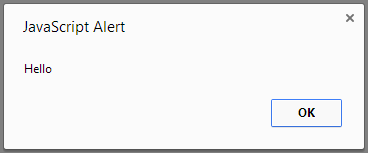
\includegraphics[width=5cm]{alert.png}
          \end{center}
    \item {\tt var input = prompt(msg)} vraagt gebruiker om invoer
          \begin{center}
            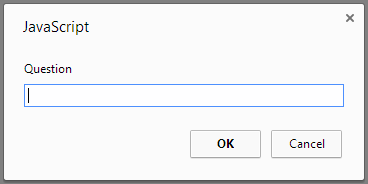
\includegraphics[width=5cm]{prompt.png}
          \end{center}
    \item {\tt var n = parseInt("123")}: omzetten string naar getal
  \end{itemize}
\end{frame}

\begin{frame}
  \frametitle{Bestaande Functies}
  \structure{Wiskunde-functies} \link{http://www.w3schools.com/js/js_math.asp}{w3schools}
  \begin{itemize}
    \item {\tt Math.sqrt}: vierkantswortel
    \item {\tt Math.floor}: afronden naar beneden
    \item {\tt Math.ceil}: afronden naar boven
    \item {\tt Math.pow}: machtsverheffing
    \item {\tt Math.abs}: absolute waarde
    \item {\tt Math.random}: genereer random getal
  \end{itemize}
\end{frame}

\begin{frame}
  \frametitle{Lokale Variabelen}
  \begin{itemize}
    \item Een functie kan lokale variabelen invoeren
    \item Tijdelijke variabelen
    \item Worden telkens opnieuw aangemaakt bij functie-oproep
  \end{itemize}
  \code[width=.4\linewidth]{locals.js}
  \begin{tikzpicture}[overlay,remember picture]
    \only<2>{
      \node[/khl/note,anchor=west] (note a) at ($ (a) + (1.5,0) $) {1};
      \draw[/khl/note arrow] (note a) -- (a);
    }

    \only<3>{
      \node[/khl/note,anchor=west] (note b) at ($ (b) + (1.5,0) $) {1};
      \draw[/khl/note arrow] (note b) -- (b);
    }

    \only<4>{
      \node[/khl/note,anchor=west] (note c) at ($ (c) + (1.5,0) $) {1};
      \draw[/khl/note arrow] (note c) -- (c);
    }
  \end{tikzpicture}
 \end{frame}

\begin{frame}
  \frametitle{Scope: Zichtbaarheid van een Variabele}
  \code[width=.4\linewidth,font size=\small]{scope.js}
  \begin{tikzpicture}[overlay,remember picture,arrow/.style={-latex,red,thick}]
    \only<2>{
      \draw[arrow] (foo ref x) to[bend right=30] (foo x);
    }
    \only<3>{
      \draw[arrow] (bar ref x) to[bend right=30] (bar x);
    }
    \only<4>{
      \draw[arrow] (qux ref x) to[bend right=30] (global x);
      \draw[arrow] (qux x) to[bend right=30] (global x);
    }
    \only<5>{
      \draw[arrow] (global ref x) to[bend right=30] (global x);
    }
  \end{tikzpicture}
\end{frame}

\begin{frame}
  \frametitle{Scope: Zichtbaarheid van een Variabele}
  \structure{Regels}
  \begin{itemize}
    \item {\tt var} verklaart dat variabele lokaal is in huidige functie
    \item Functie kan aan ``buitenliggende'' variabelen
    \item Buiten functie F kan men niet aan lokale variabelen van F
  \end{itemize}

  \vskip5mm
  \structure{Java vs JavaScript}
  \begin{itemize}
    \item Regels verschillen tussen Java en JavaScript
    \item JavaScript regels eigenwijs, complex en onintu\"itief
    \item Exacte JavaScript regels hoef je niet te kennen
    \item Vuistregel: scope werkt per functie, gebruik altijd {\tt var}
    \item Java regels moet je w\'el goed kennen (komen immers overeen met regels van andere talen)
  \end{itemize}
\end{frame}

\begin{frame}
  \frametitle{Globale Variabelen}
  \begin{itemize}
    \item Globale globale variabele = variabele buiten functie
    \item Sterk afgeraden!
    \item Zorgt dat ongerelateerde stukken code kunnen interferen
    \item Niet modulair
    \item Leidt snel tot moeilijk te vinden bugs
  \end{itemize}
  \vskip5mm
  \code[width=.5\linewidth]{globals.js}
\end{frame}

\begin{frame}
  \frametitle{Analogie: Met Lokale Schalen}
  \code[font size=\small,width=.95\linewidth]{recipe.js}
\end{frame}

\begin{frame}
  \frametitle{Analogie: Met Globale Schaal}
  \code[font size=\small,width=.95\linewidth]{recipe2.js}
\end{frame}

\begin{frame}
  \frametitle{Analogie}
  \begin{itemize}
    \item Met lokale schalen: chocolade en deeg in aparte schalen
          \vskip4mm
    \item Met globale schaal: alles zit in \'e\'en schaal, recept mislukt
          \vskip4mm
    \item Mogelijke oplossing: aparte schaal per handeling
          \begin{itemize}
            \item Veel globale schalen nodig
            \item Zouden allemaal verschillende namen nodig hebben
            \item Zou veel plaats in beslag nemen
          \end{itemize}
          \vskip4mm
    \item Idem voor variabelen
  \end{itemize}
\end{frame}


% Waarom functies: herbruik, abstractie, modulariteit

\end{document}

%%% Local Variables: 
%%% mode: latex
%%% TeX-master: t
%%% End: 
